\section{Compiler}

Creating a binary executable from C++ code is a multistage process that can be
divided into two major steps: compiling and linking. Each of these steps goes
through a magnitude of sub-routines whose end goal is to produce a binary executable
file that is used to run the main application. Alternatively, compilers are also
capable of creating a static or shared library that can be used in other projects.
Prominent examples include, amongst other things:

\begin{itemize}
    \item \textbf{Boost:} a set of 164 individual libraries that range from Algorithm
    to YAP, an expression template library for C++14 and later.
    \item \textbf{STL:} a standard template library.
    \item \textbf{QT:} a tried-and-tested template library.
    \item \textbf{SFML:} a simple and fast multimedia library living up to its name.
    \item \textbf{OpenCV:} a high-performance image processing library.
\end{itemize}

There are many C++ compilers out there, but the ones most commonly used probably are:

\begin{itemize}
    \item Clang
    \item GCC
    \item MSVC
    \item Intel C++ Compiler
\end{itemize}

The main purpose of a compiler is to translate a high-level language into a transient
lower-level language, for example assembly. In \autocite{wirth1996}, a compiler is
defined as a program that automatically translates a program text into a suitable
instruction sequence before it is processed by a computer where the text to be
translated is called source code (or sometimes source text). Note that some compilers
don't use an assembler in an intermediate step at all, but rather directly emit
byte code into an object file. In the simplest terms, an object file consists of
three things:

\begin{itemize}
    \item Ranges of unsplittable data (sections and atoms)
    \item Names that define or reference data (symbols)
    \item Lists of modifications to data (relocations)
\end{itemize}

In many cases the compiler is able to produce more efficient assembly code than
if it were handwritten. One of its main responsibilities is to ensure that the code
follows the rules of the C++ programming language. During this step the compiler
also performs a series of optimization techniques where applicable (inter alia
constant folding and function inlining) before the assembler transforms this intermediate
product into object code. Bear in mind that many compilers turn off all optimizations
by default to improve the debug experience. They're the penultimate result of the
build process and contain machine code with unresolved external dependencies that
are fed into the linker in the next stage. Some compilers provide support for multiple
languages or target architectures which is one of the many compelling reasons to
use them over others. In comparison, a traditional static compiler uses a three-phase
design whose major components are the frontend, optimizer and the backend \autocite{lattner2011}.

\begin{itemize}
    \item \textbf{Frontend:} Performs lexical and syntax analysis as well as type
    checking, the result of which is the abstract syntax tree (AST) that represents
    the structure of the source text.
    \item \textbf{Optimizer:} Derives information from the intermediate code
    representation (IR) in order to recognize instructions that can be replaced
    with functionally equivalent optimizations.
    \item \textbf{Backend:} Generates machine-dependent optimizations (for example
    peephole optimizations in assembly). This code targets a specific CPU architecture. 
\end{itemize}

\begin{figure}[hbt!]
    \centering
    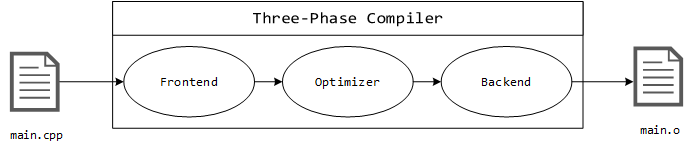
\includegraphics[width=1\textwidth]{images/ThreePhaseDesign.png}
\end{figure}

LLVM takes this design to the next level by implementing a modular compiler system
that provides an interface for many different languages. The advantage of this design
is the common optimizer that can be repurposed for different compiler frontends,
while also redirecting development efforts into a single component which further
increases the quality of the compiler that is now backed by a larger community.

\begin{figure}[hbt!]
    \centering
    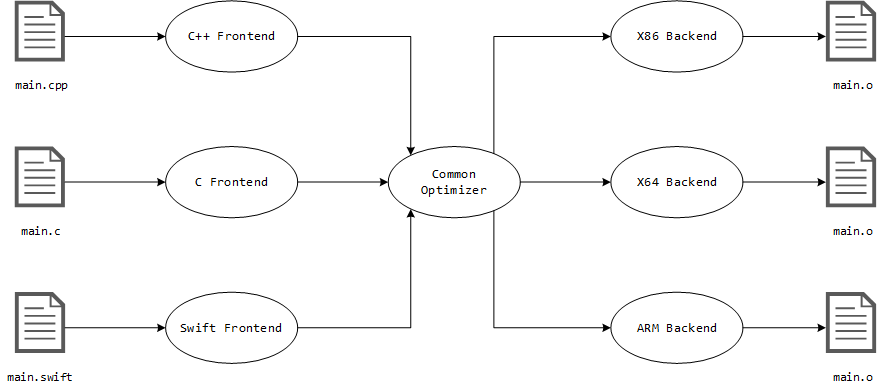
\includegraphics[width=1\textwidth]{images/ThreePhaseDesignRetargeting.png}
\end{figure}

There are other reasons why commercial application developers would prefer LLVM
over other compilers such as GCC: it is licensed under a BSD-style Apache License
v2.0 as opposed to GCC v4.3+ which uses the less permissive copyleft GPLv3 license
that is not viable for propriety projects \autocite{fandrey2010}. However, this is
not the decisive factor for small applications written by independent developers
or students. In many cases, using the GPLv3 license for a project would be more
beneficial for the open-source software community\footnote{For a more thorough
explanation visit \url{https://www.gnu.org/licenses/rms-why-gplv3.html}.}.

Most compilers provide a set of increasingly performant optimization options that
can be controlled by explicitly enabling their respective flags. Starting with v11.0,
Clang has changed its optimization flags to match the defaults of GCC. In case of
Clang, it defines these flags as followed\footnote{See also this \url{https://clang.llvm.org/docs/CommandGuide/clang.html}
for a comprehensive list of command line options.}:

\begin{itemize}
    \item \texttt{-O0:} On this level, no optimization pass is enabled. It compiles
    the fastest and generates the most executable code.
    \item \texttt{-O1:} Somewhere between \texttt{-O0} and \texttt{-O2}.
    \item \texttt{-O2:} Moderate level of optimization which enables most optimizations.
    \item \texttt{-O3:} Like \texttt{-O2}, except that it enables optimizations
    that take longer to perform or that may generate larger code (in an attempt
    to make the program run faster).
    \item \texttt{-Ofast:} Enables all the optimizations from \texttt{-O3} along
    with other aggressive optimizations that may violate strict compliance with
    language standards.
    \item \texttt{-Os:} Like \texttt{-O2}, with extra optimizations to reduce code size. 
    \item \texttt{-Oz:} Like \texttt{-Os} (and thus like \texttt{-O2}) but reduces
    code size further.
    \item \texttt{-Og:} Like \texttt{-O1}. In future versions, this option might
    disable different optimizations in order to improve debuggability.
    \item \texttt{-O:} Equivalent to \texttt{-O1}.
    \item \texttt{-O4:} Currently equivalent to \texttt{-O3}.
\end{itemize}

Building projects for release purposes is a whole topic on its own and is not going
to be covered in this document in any more detail. 
